\documentclass[11pt]{article}
\bibliographystyle{plain}
\usepackage{geometry} % see geometry.pdf on how to lay out the page. There's lots.
\usepackage{amsmath,amssymb} 
\usepackage{epsfig,epsf,subfigure}
\geometry{a4paper} 


\begin{document}
 
\LARGE
\begin{center}
TMA4280: Introduction to Supercomputing
\end{center}
\vspace{0.5in}

\begin{center}
{\bf Problem set 6}
\end{center}

\Large
\vspace{0.5in}
\begin{center}
Spring 2015
\end{center}

\vspace{0.5in}

{\bf NOTE THAT}:
\begin{itemize}
\item this exercise is mandatory;
\item you can work on this problem alone or with up to two other students;
\item a report describing the solution should be written (max 12 pages);
\item please write your \emph{name(s)} on the report; 
\item please include the source code as separate files rather than inline in the report (save the forest!)
\item please make sure that you have answered all the questions; 
\item the due date is Friday, April 10, 2015;
\item the report will count 30\% towards the final grade.
\end{itemize}

\vspace{0.5in}

\begin{center}
\copyright Einar M. R{\o}nquist \\
Department of Mathematical Sciences\\
NTNU, N-7491 Trondheim, Norway\\
All rights reserved
\end{center}

\large

\newpage


Consider the solution of the two-dimensional Poisson problem
\begin{eqnarray}
-\nabla^2 u & = & f \hspace{.5in} \textrm{in} \,\,\, \Omega = (0,1)\times (0,1) \\
u & = & 0 \hspace{.5in} \textrm{on} \,\,\, \partial\Omega\, .
\end{eqnarray}
Here, $f$ is a given right hand side and $u$ is the solution.

Assume that we discretize this problem on a regular finite 
difference grid with $(n+1)$ points in each spatial direction.
Hence, the mesh spacing $h=1/n$. We use the standard 5-point 
stencil to discretize the Laplace operator. 

In order to solve the system of algebraic equations, 
we apply the diagonalization methods discussed in class.
In particular, we apply the Discrete Sine Transform (DST) 
in order to obtain a solution of this problem in 
${\cal O}(n^2\log n)$ floating point operations.

\begin{description}
\item a) Write a program to solve the Poisson problem 
on $p$ processors using the algorithms described above.
You can choose $f=1$ for the initial development.

Use the provided routines to compute the DST and its inverse 
based on FFT. See Appendix A for details on compiling, linking 
and running the {\em serial} version of the Poisson solver. 
Use the MPI communication library in order to 
develop your program for distributed memory 
parallel computers, and OpenMP to utilize $t$ threads in each MPI process.
See Appendix C for comments on the transpose operation. 

\item b) Run your parallel program on \texttt{kongull}, the 
cluster at NTNU. \\Obtain detailed timing 
results for different combinations of $n = 2^k$ and $p, t$. \\
%Note that your program should function for {\em any} number of processors. \\ 
In particular, you should demonstrate that your 
program functions correctly for (selected) values of $p$ in 
the range $1 \le p\le 36$. \\
Follow the procedure described 
in Appendix B.
 
{\bf Note 1}. Having available a program that runs
extremely fast is of no use unless the final answer is correct.

{\bf Note 2}. It is sufficient 
(and strongly recommended!) that you test the correctness of 
your program on a {\em small} problem size before solving 
larger problems. 

%{\bf Note 3}. For $p\leq 16$ it is possible to run your program  interactively. 


\item c) 
Run your program with $n=16384$ and $p*t=36$,
i.e., solve the Poisson problem with about 270 million grid points on 36 processors. 
Does the hybrid model work better, worse or equivalent compared to the pure
distributed memory model? Explain your observations.

\newpage

\item d) Report the speedup, $S_p$, as well as the parallel efficiency, $\eta_p$, for 
different values of $n$ and $p$. 
The parallel efficiency on $p$ processors is defined as $\eta_p = \frac{S_p}{p}$. \\
%Discuss your findings.  
%For example, 
How do your timing results scale with the problem size 
$n^2$ for a fixed number of processors? Is the scaling as expected?
Do you see an improved speedup if you increase the problem size? 

{\bf Note 4}: 
%Even though you may develop a correctly working parallel program 
%in an interactive mode, you {\it have to} do all your your timings in batch mode, i.e., 
You need to submit your individual jobs to a batch queue. 
This is very important on supercomputer systems because this is the only way to ensure 
consistent and reliable timing results. 

\item e) Modify the given data $f$ to be a function of 
your own choice. As an example, you could choose $f$ to be 
a smooth function like 
$f(x,y) = e^{x}\cdot \sin(2\pi x)\cdot \sin(\pi y)$. 
Another example is to let $f$ represent 2 point sources,
e.g., $f=0$ in the whole domain except at 2 chosen (grid)points 
$(x_1,y_1)$ and $(x_2,y_2)$ inside the domain where 
$f(x_1,y_1) = 1$ and $f(x_2,y_2) = -1$. 

Run your program with the new 
right hand side $f$ for a particular $n$ and a particular $p$. 
Do you have to modify anything related to the parallel 
implementation when you change $f$, i.e., when you solve 
a different Poisson problem?

\item f) Discuss how you would modify the numerical 
algorithm to deal with the case where $u\neq 0$ on 
$\partial\Omega$, i.e., in the case of non-homogeneous 
Dirichlet boundary conditions. You do not have to implement this.

\item g) In this exercise (as well as in the lectures), 
we have assumed that the domain is the unit square,
i.e., $\Omega = (0,1)\times (0,1)$. 
Discuss how you would modify the Poisson solver based
on diagonalization techniques if the domain $\Omega$ instead 
is a rectangle with sides $L_x$ and $L_y$, i.e.,
$\Omega = (0,L_x)\times (0,L_y)$.
You can still assume a regular finite difference grid with 
$(n+1)$ points in each spatial direction. Does this extension 
of the original method change anything in terms of your 
parallel implementation? You do not have to implement this case.

\end{description}
\newpage
\textbf{\textit{General comments:}}
\begin{quote}
    It will in general be emphasized that the program is well
    parallelized and load balanced. It will further be of importance
    that the program is well organized. It is allowed to use more
    memory than the minimum required, if it speeds up the program,
    but this should be done with care.

    A report describing results of parallelization of a scientific
    problem typically contains:
    \begin{itemize}
    \item a description of the mathematical/numerical problem,
    \item a discussion of possible solution strategies,
    \item a short explanation of the finished program,
    \item description of the parallel computer on which the numerical
        results were obtained, which compiler and compiler options
        you used to compile the program, as well as any other relevant
        information such as sublibraries utilized,
    \item numerical results (preferably plot(s) of the
        result(s)),
    \item analysis (both theoretical and experimental) of the
        performance of the algorithm and implementation (time usage,
        speedup and efficiency as a function of problem dimension and
        number of processors),
    \item a discussion of bottlenecks and possible
        optimization, and
    \item possibly a listing of the relevant parts of the source code
        in the appendix.
    \end{itemize}
\end{quote}


\noindent {\bf APPENDIX A. Compiling and linking}
The serial code ships with a CMake based build system for portability
and simplicity. You can generate a build system using
\begin{verbatim}
  module load intel/compilers/11.1.059
  module load cmake
  CC=icc FC=ifort cmake . -DCMAKE_BUILD_TYPE=Release
\end{verbatim}
assuming you are located in the folder with the shipped CMakeLists.txt.
This will, on success, generate a Makefile, and you can then build
and run the program using
\begin{verbatim}
make
./poisson 128
\end{verbatim}
The first statement builds the program, while the second statement
runs the code on a single processor with $n=128$.
Note that $n$ needs to be a power of 2 in order to use 
the discrete sine transform provided here. Note that by default CMake
will not show you the compiler commands. You can see these by doing
\begin{verbatim}
make VERBOSE=1
\end{verbatim}

\vspace{.3in}


\noindent {\bf APPENDIX B. Verification of correctness}

One way to verify that the code works correctly is to do 
a {\em convergence test}. Following this approach, we first assume 
an exact solution to our Poisson problem. For example, we can assume 
that the exact solution is given as 
\begin{equation}
u(x,y) = \sin(\pi x)\cdot \sin(2\pi y) .
\end{equation}
This solution satisfies the homogeneous boundary conditions 
$u=0$ on $\partial\Omega$. 

Next, we evaluate $-\nabla^2 u$ which should be equal to $f$, i.e.,
\begin{equation}
f(x,y) = -\nabla^2 u = 5\pi^2\cdot \sin(\pi x)\cdot \sin(2\pi y) .
\end{equation}
Assuming the given data $f(x,y)$ as specified in (4), we now solve the 
Poisson problem numerically. We then compare the numerically computed
solution with the exact solution at the finite difference points. 
The maximum pointwise error should then decrease to zero as ${\cal
  O}(h^2)$, i.e., if we increase $n$ with a factor of two (or 
equivalently, decrease $h$ with a factor of two), the error should 
decrease with a factor of four. 
Remember that finding the maximum pointwise error using multiple 
processors will require communication!
%\vspace{1.0in}

\noindent {\bf APPENDIX C. Comments on the transpose operation}

The implementation of the transpose operation is trivial in a 
serial context. In a parallel context, using a distributed 
memory programming model, message passing has to be used. 
In this case, the transpose of a matrix will involve all-to-all 
communication. 

Part of the solution algorithm in this exercise requires 
a parallel implementation of the transpose operation. 
We have given a matrix of a certain dimension. 
We can distribute the matrix such that each processor 
is responsible for a certain number of columns (or rows). 

The most convenient way to implement the transpose operation 
is to use the MPI library function \textrm{MPI\_ALLTOALLV} in FORTRAN 
(or \textrm{MPI\_Alltoallv} in C);\\
see Figure 1. For a detailed description of this function, 
see reference 1, page 174, or simply input the function name into an internet
search engine.

\vspace{1.in}

{\bf Reference}\\
\\
1. Snir, Otto, Huss-Lederman, Walker, and Dongarra,\\
{\em MPI: The Complete Reference}, The MIT Press, Cambridge, MA.

 \begin{figure}[htbp]
  \begin{center}
    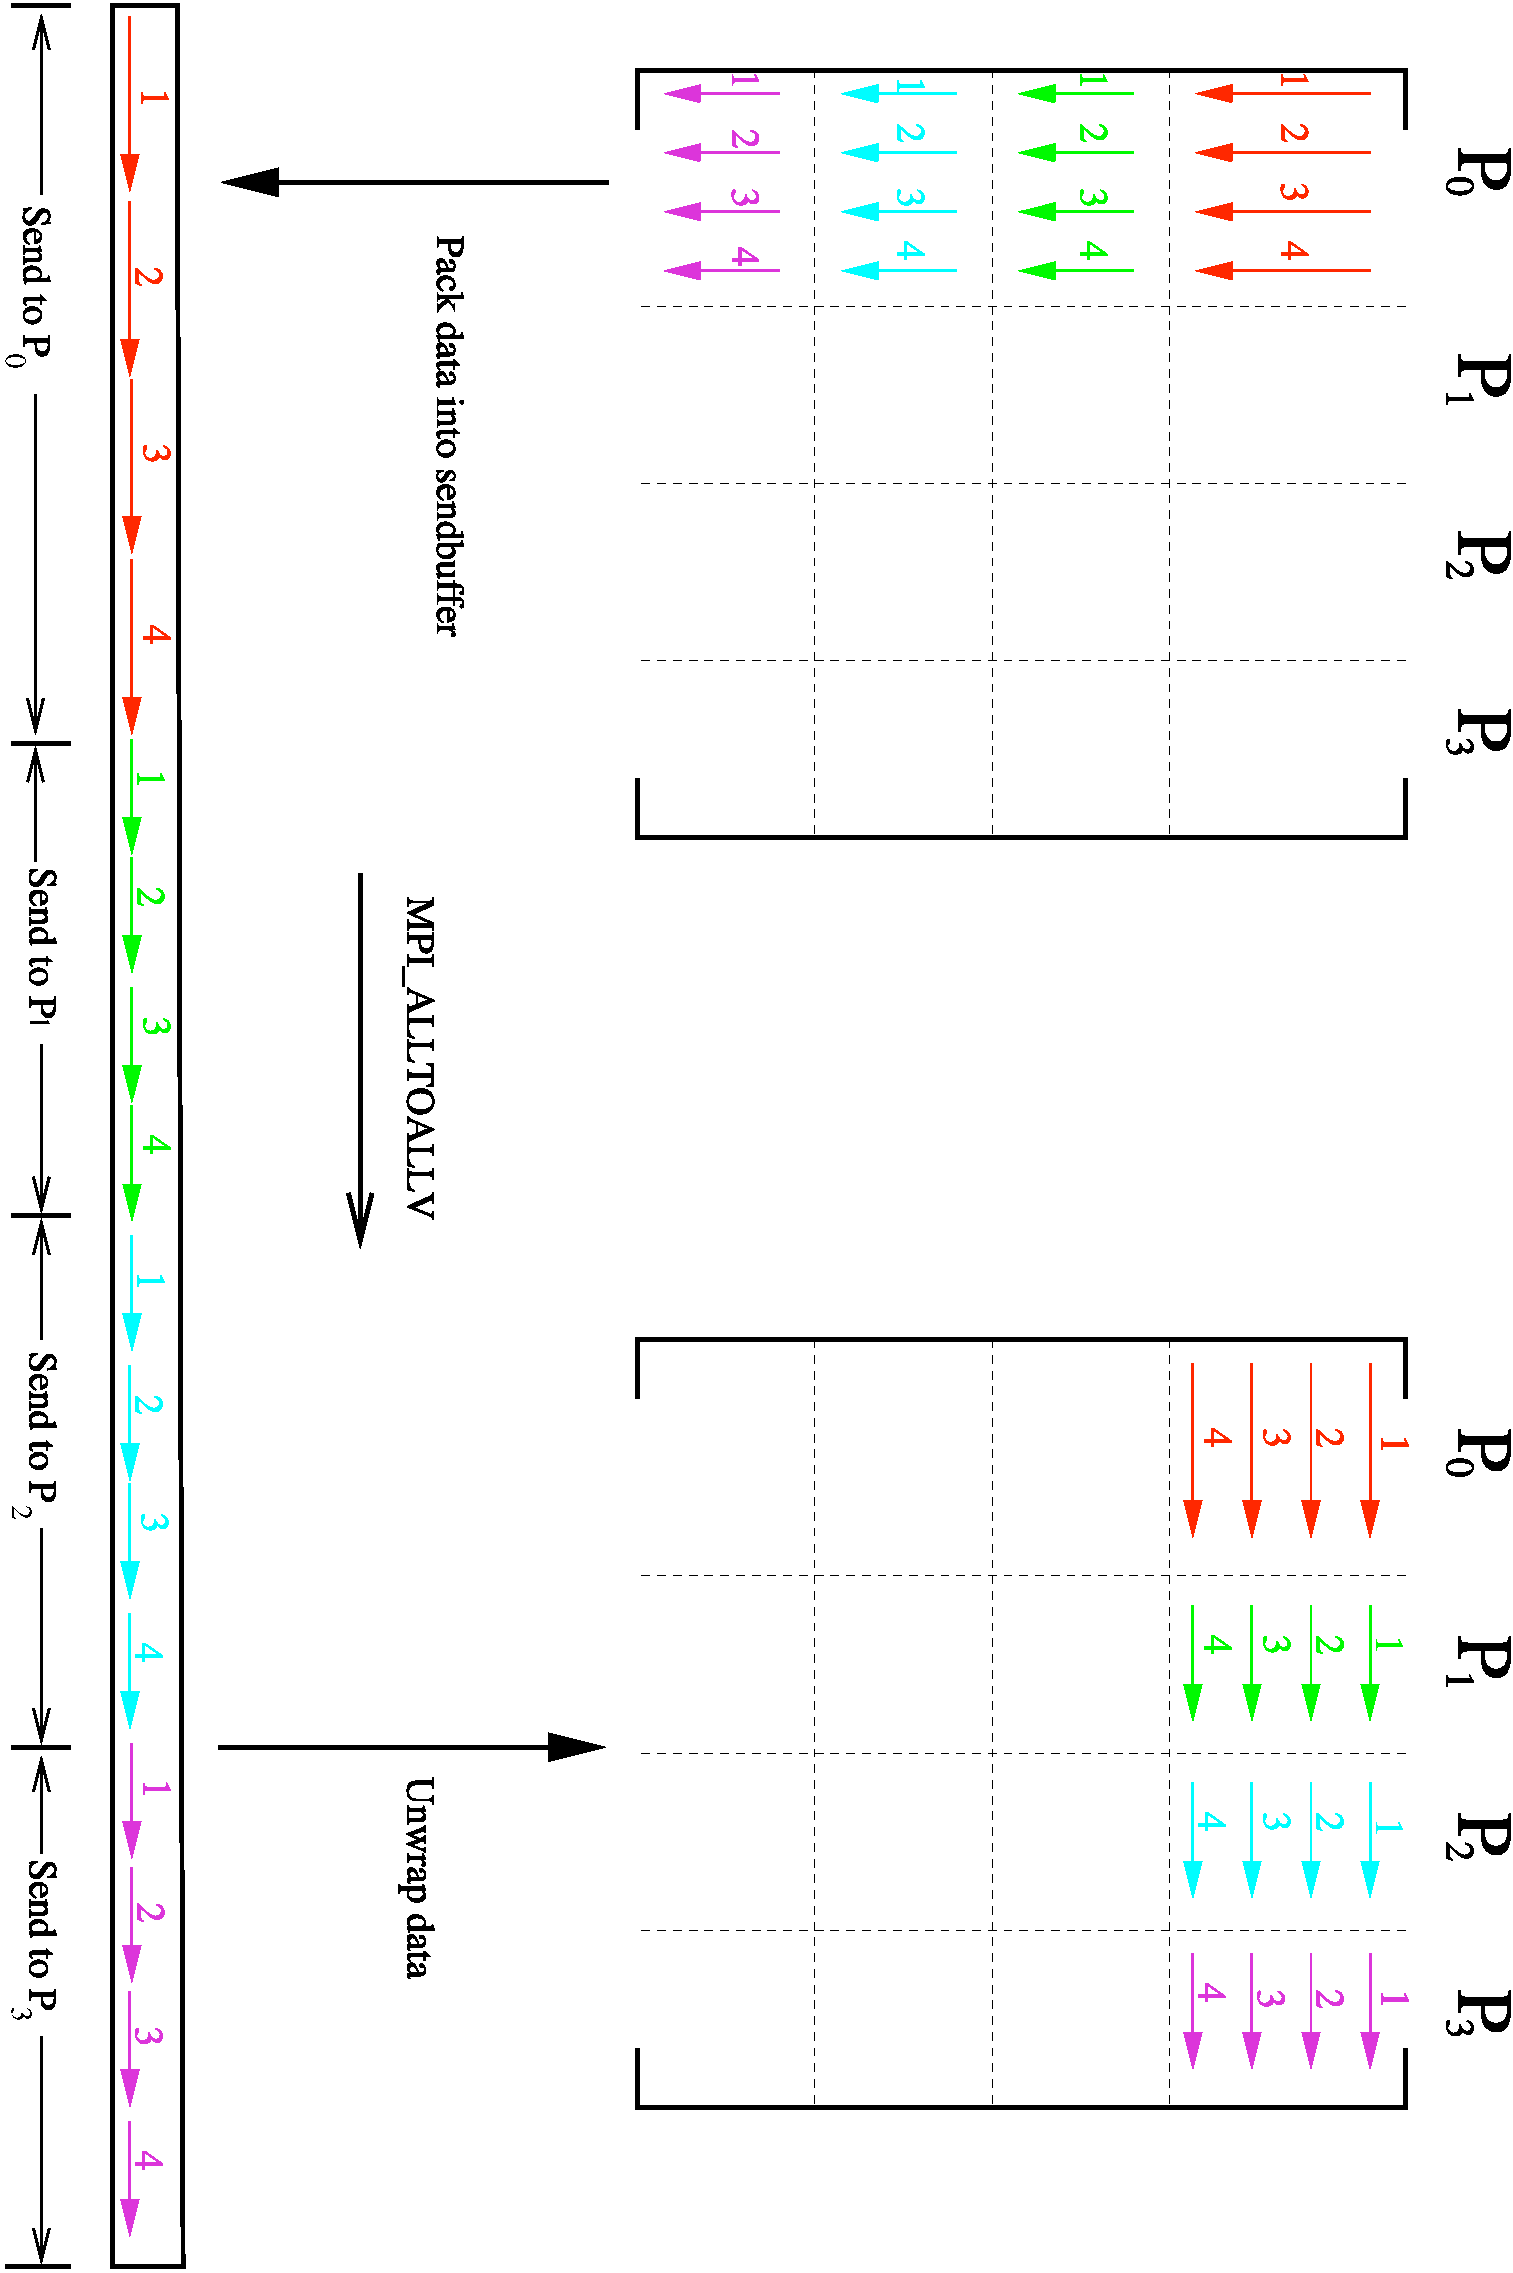
\includegraphics[scale=0.6]{matrix_blocktranspose}
  \end{center}
  \caption{
The transpose operation using message passing: 
the packing and unpacking of data.
The figure is due to Bjarte H{\ae}gland.
}
\label{}
\end{figure}

\end{document}

